\documentclass[class=book, crop=false]{standalone}
\usepackage[utf8]{inputenc}
\usepackage[subpreambles=true]{standalone}
\usepackage{import}
\usepackage[ruled,vlined]{algorithm2e}

\usepackage{amsmath}
\usepackage{amssymb}
\usepackage[margin=1.2in]{geometry}
\usepackage[sorting = none,
            doi = true  %lesedato for url-adresse
            ]{biblatex} %none gir bibliografi i sitert rekkefølge
\addbibresource{reference.bib}
\usepackage{csquotes}
\usepackage{pgfplots}
\pgfplotsset{compat=1.15}

\begin{document}
\chapter{Problem Description}\label{chap:problem_description}
Solar power production occurs during day-time and is, not surprisingly, controlled by the sun. As photovoltaic modules become more prevalent in residential areas, they will grow to a size where they produce a significant amount of power that must be transported out on the grid. In the afternoon, power must be imported from the external grid because the solar power production is low when residential areas consume power. A consequence of this is that safety bounds for both voltage and line capacity are in danger of being violated. A strategy for avoiding is called demand response. Albadi and El-Saadany give the following definition of demand response \cite{demand_response_definition}:

\begin{displayquote}
Demand response can be defined as the changes in electricity usage by end-use customers from their normal consumption patterns in response to changes in the price of electricity over time. Further, DR can be also defined as the incentive payments designed to induce lower electricity use at times of high wholesale market prices or when system reliability is jeopardised. DR includes all intentional electricity consumption pattern modifications by end-use customers that are intended to alter the timing, level of
instantaneous demand, or total electricity consumption.
\end{displayquote}


The idea is to modify the demand of electric power to follow the production profile of distributed energy resources (DER), such as solar power. The consequence of this is that the solar power is consumed locally instead of having to be transported out to the grid, through lines that originally were not constructed for DER. Vázquez-Canteli and Nagy list the following advantages of demand response \cite{active_network_management}:

\begin{itemize}
\item Improved grid stability due to increased demand flexibility. 
\item Shift of peak demand towards periods of peak renewable energy
generation.
\item Lower thermal costs and electricity prices. Since the peak to average
ratio of the demand decreases, less peaking plants need to be operated. 
\item Reduction of the investments in generation, transmission, and distribution assets, which are sized to meet peak demand.
\item Lower capacity reserves requirements.
\item Reduced energy bills for consumers. 
\end{itemize}


Demand response can be categorised into two main programs: Price-Based Programs and Incentive-Based Programs (IBP) \cite{demand_response_definition}. This thesis will investigate the latter program (IBS) by directly controlling the loads around in the grid. There are several published papers that uses reinforcement learning to achieve demand response \cite{active_network_management}. Typically they try to control individual thermostatic loads, such as heat pumps and electric water heaters, in a categorical on-off setting. The scope of this thesis is not to control individual power consuming units, but to continually control the absolute load at different buses in a power grid, given some flexibility at that bus. It might seem strange to use continuous control since power consuming units generally can not be set to an arbitrary power level. The nature of a power component is binary: it either consumes power or it does not consume power. Consequently, a valid question is whether a continuous control setup even is realisable in a real power system. Although individual power consuming units are binary, a large collection of units connected to a bus can be approximated as continuous. Imagine 1000 households connected to a bus and that each household has several power consuming components that can be controlled, such as electric vehicles, water heater and heat pumps. Assuming these units have some flexibility in terms of consumption, it is possible to control all these devices in such a way that they appear continuous at the bus. This thesis will assume that a system for turning on and off the individual power consumers already exist, so the centralised agent can consider the loads continuous in some interval of flexibility. This assumption can be said to be unrealistic, but the scope of this thesis is to test continuous demand control at buses experimentally, under some ideal assumptions. The advantage of this setup is that the action space of the algorithm is dramatically reduced, as there is only one action per bus in the grid. Controlling individual components in a power grid quickly gives a very large and impractical action space. The set of possible actions doubles for every additional control device, and exponential growth is hard to tackle, even for modern computers.

The specific setup in this thesis is based on several assumptions for a hypothetical future power grid. The electrical power grid used is constructed by the International Council on Large Electric Systems (CIGRE) as a benchmark network that can be used for analysis of DER integration \cite{cigre}. The network is predefined in \texttt{pandapower}, the Python module used for power flow calculations, and can be defined with different renewable energy sources connected at different buses. The grid used is visualised in figure \ref{fig:problem:cigre_network}. 

\begin{figure}[ht]
    \center
    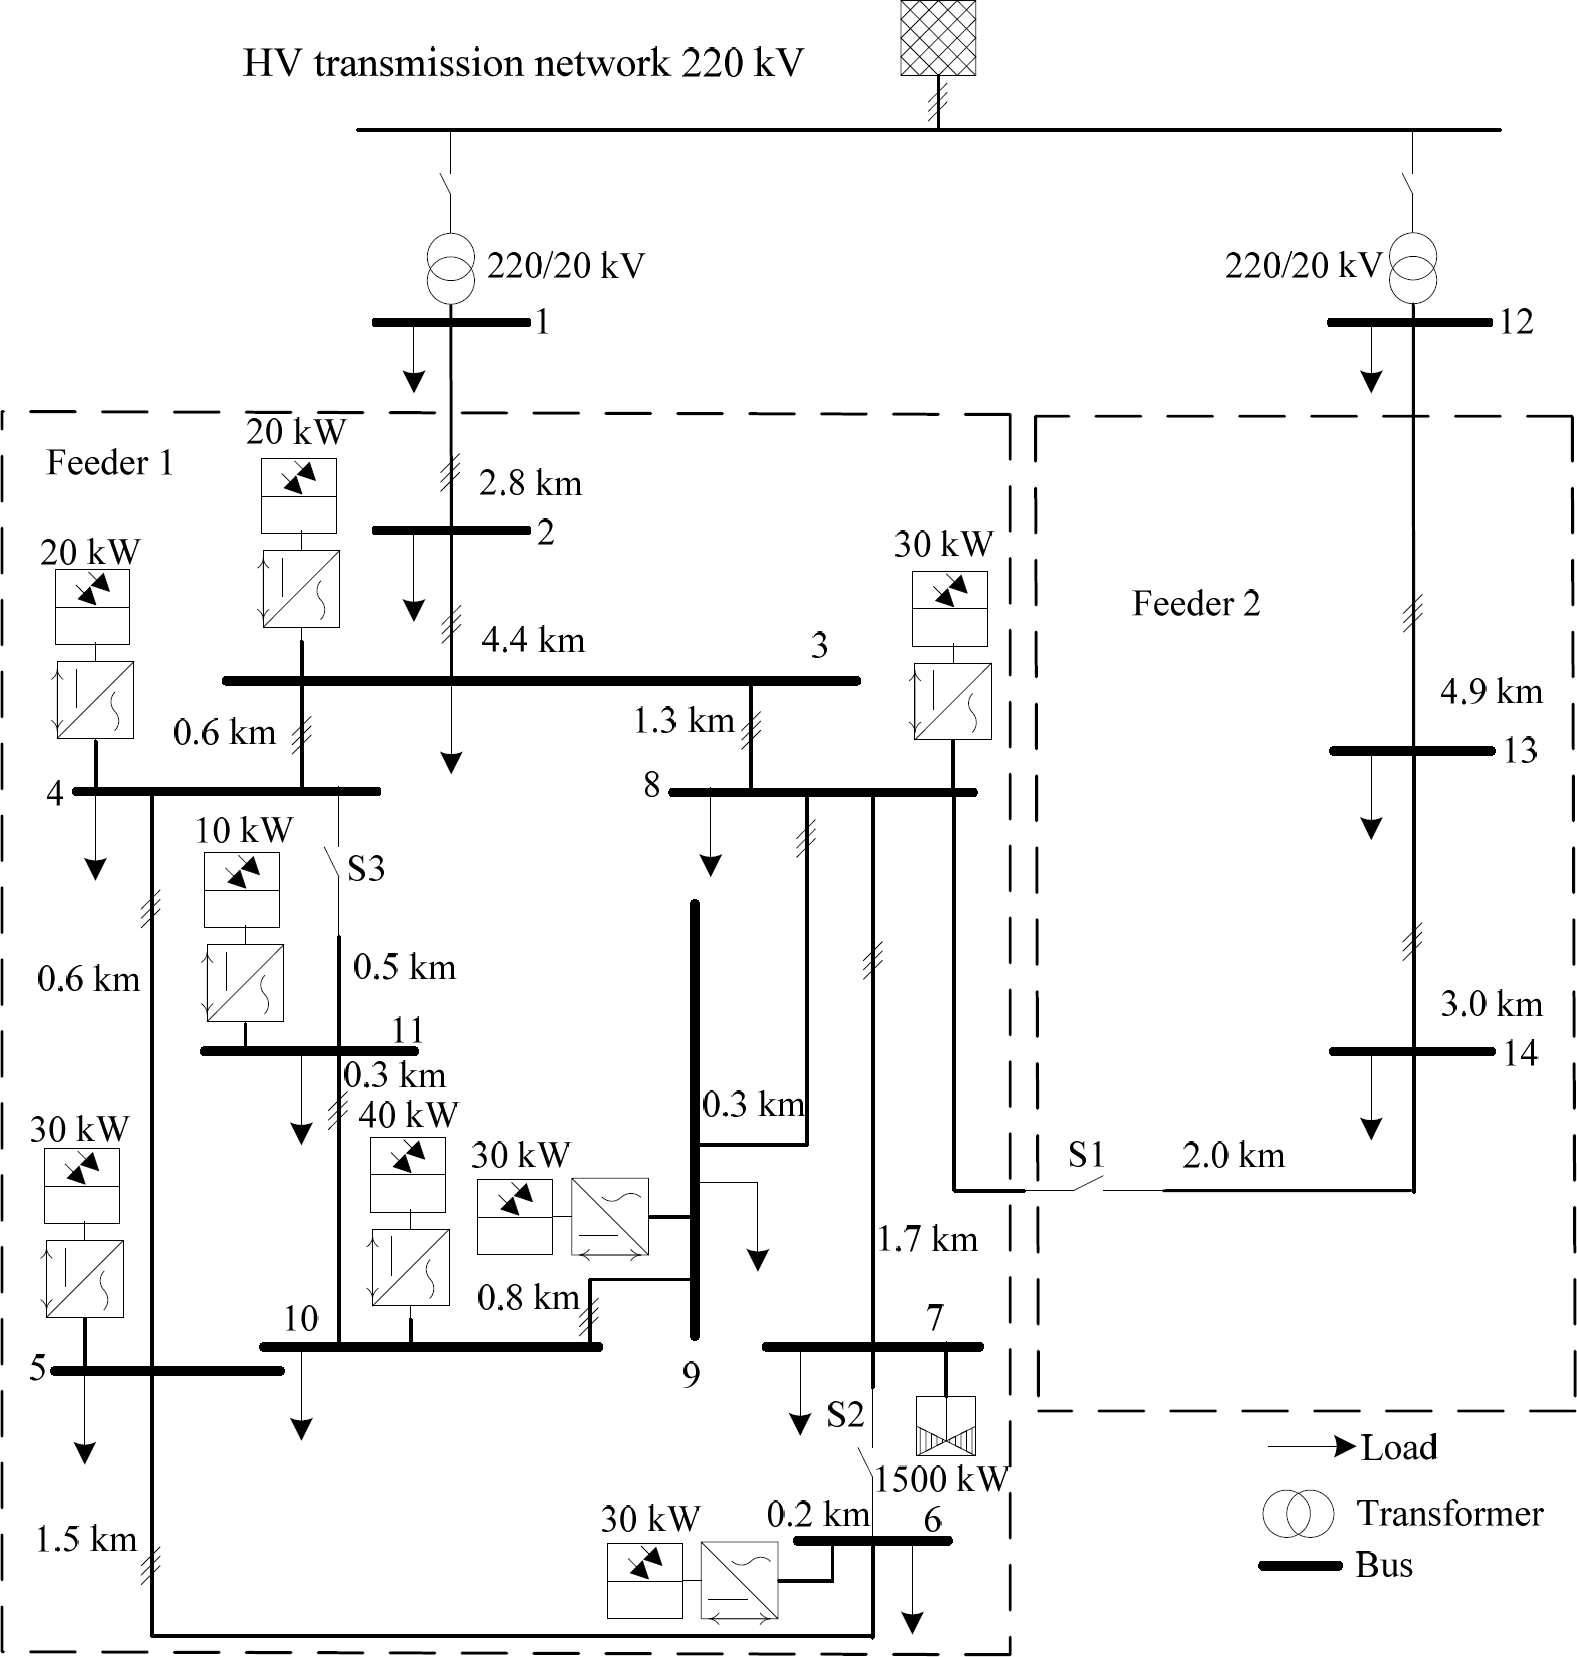
\includegraphics[height=14cm, width=13.5cm]{figures/cigre_network_mv_der.png}
    \caption[size = 9]{CIGRE network with solar and wind power that is used in the reinforcement learning algorithm \cite{cigre}}
    \label{fig:problem:cigre_network}
\end{figure}


The left-most feeder has several solar producing units connected and wind power connected to bus 7. From a power flow perspective, there is no difference between a wind farm (without voltage regulation) and solar production. They are both modelled as static generators (PQ-node). For simplicity, the wind farm connected at bus 7 is assumed to be solar in this thesis, i.e its power production follows the sun profile through the day. The time resolution in this task is chosen to be hourly. In other words, the demand and solar production at every bus is updated every hour, and assumed constant in between hours. The demand profile is generated using \textit{enlopy}, a python toolkit for energy demand time series \cite{enlopy}. The demand signal is generated based on data of the energy consumption of private households.

A data set with satellite-derived solar irradiance in central Norway is used as input to define the production of solar power \cite{solar_data}. Figure \ref{fig:problem:solar_data} plots a time series of the solar irradiance, and a couple of example days. The solar data is scaled so the maximum value is 1.

\begin{figure}[ht]
    \center
    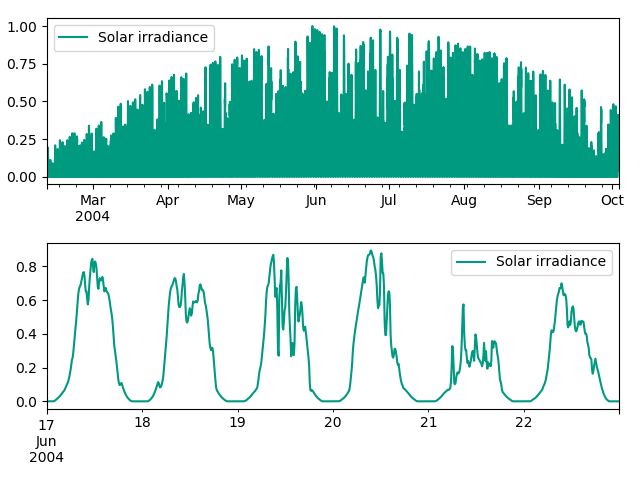
\includegraphics[height=9cm, width=13.5cm]{figures/solar_data.png}
    \caption[size = 9]{The solar irradiance data used in the reinforcement model. The period is 2004-02-11 to 2004-10-03, generated from SoDa \cite{solar_data}. (lon,lat) = (63.395,10.381) }
    \label{fig:problem:solar_data}
\end{figure}



The signal of solar production and power demand is assumed equal at all buses and scaled up based on nominal values of the loads at each bus. Note that the nominal values vary a lot from bus to bus. For instance, if the demand signal is 0.5, the consumption at each bus is determined by multiplying 0.5 with their respective nominal power. The same is true for the generation of solar power. This reduces the state space, as there is no need for a unique demand forecast for all the loads.  For simplicity, the power factor is assumed constant at every bus, meaning the reactive power at each load is a percentage of the active power at all times. The power factor at each load is the same as the default values in the CIGRE network. The values of the solar production are intentionally amplified so that the safety margins for line current and voltage magnitudes in the grid frequently are violated if no actions are taken. The solar producing units do not output any reactive power, only active power. 

All loads have an hourly forecast of energy consumption that is used to update the active and reactive powers at every time step. It is assumed that the loads at all buses have some flexibility, say 10 \% of the actual demand, that can be centrally controlled at every hour.

\section{Network variables}
The CIGRE network shown in figure \ref{fig:problem:cigre_network} is the power net the reinforcement algorithm is control. The number of components are summarised in table \ref{table:cigre_components}

\begin{table}[ht]
\centering
\caption{Component in the CIGRE network}
\label{table:cigre_components}
\begin{tabular}{l|ll}

Component  & Symbol & Amount 
\\ 
\hline
Bus & N & 15 \\
Switch & - & 8 \\
Static generator & G & 9 \\ 
Line & L & 15 \\
Load & F & 18 \\
Transformer &- & 2

 \\
\hline
\end{tabular}
\end{table}
Table \ref{table:cigre_components} shows that there are 18 loads and 15 buses in the system. The reason is that there are several load elements connected to some buses which makes the number of loads greater than the number of buses.  



\section{State space}\label{section:problem:state_space}
It is not obvious how to design the state space for the agent. This section presents several spaces that could be useful for the reinforcement algorithm. Let $\mathcal{S}_{sun} \subseteq  \mathbb{R}^{H}$ be space of the forecasted total solar production in the grid \textit{H} hours into the future . This gives the agent information about the coming solar production in the power marked that can be used for finding strategies. For instance, consider a situation with a high production of solar power that is overreaching the capacity in the power lines. If the agent sees that there is a dip in solar production in the next hour due to clouds, it can increase the local demand at solar producing, to relieve the overloaded power lines. It can then safely decrease the demand the next hour, since the sun is blocked by the clouds. This is an example of a desired behaviour that the agent ideally should find. The buses are assumed to be geographically close, so the solar irradiance is the same. If a cloud blocks the sun at bus 1, then it also blocks the sun at all the other buses in the system. This significantly reduces the state space compared to a unique forecast for every bus. 


Let $\mathcal{S}_{demand} \subseteq \mathbb{R}^{F\cdot H}$ be the space of the forecasted power demand $H$ hours into the future in a grid with $F$ flexible loads. It is also possible to let the total demand in the market represent the demand state. A problem with this approach is that it only partially describes the demand situations in the marked since the agent does not receive information about demand at individual loads. An advantage, however, is that the size of the a state vector from  $\mathcal{S}_{demand}$ is much smaller than a corresponding vector for all loads. Specifically, the CIGRE network that is used has 18 loads that would make the state vector 18 times greater.



Let $\mathcal{S}_{bus} \subseteq \mathbb{R}^{4N}$ be the space representing the state of all the buses in the net. Specifically

\begin{equation}
   \begin{aligned}
   \label{eq:problem:bus_state}
\mathcal{S}_{bus} = \{|V_{i}|, \delta_{i}, P_{i}, Q_{i} |\; i = 1,...,N\}
    \end{aligned} 
\end{equation}

where $|V_{i}|,\delta_{i}, P_{i}$ and $Q_{i}$ respectively are the voltage magnitude, voltage phase angle, active power injection and reactive power injection at bus $i$ in a $N$-bus system. This could give information to the agent about how stressed the system is. For instance, large values for active power $P_{i}$ and voltage magnitude $|V_{i}|$ indicate a stressed situation at bus $i$ possibly due to high solar production. 



The agent should also get information that ensures that the consumption at a load merely is shifted and not altered in absolute magnitude. In other words, a state that contains information about the energy balance in the grid. A positive energy balance means that the agent has forced the loads to use more energy than the real demand. If the agent changes a load by -1 MW for an hour, the agent should ideally increase the load by 1 MW some time not far into the future. Gemine et al did this by making a commitment when a load is modulated. When a load is modulated, it follows a predefined modulation curve for $T_{d}$ time steps (for instance 4 steps) \cite{active_network_management}. The modulation signal is constructed so that is sums to zero of over the time period $T_{d}$, which guarantees that the total energy consumption of the load is constant. This could be a possible approach for a reinforcement learning algorithm as well. The state vector could indicate in what modulation step a load is at. For instance, if the modulation started at $t_{0}$ for a load and the current time step is $t_{0} + 3$, then the load component of this vector is 3. The agent is then always fed with a signal that tells it the commitment stage of that load. The desired action of the agent at a time step in the commitment period will simply be ignored so that the load follows the modulation signal. This has the drawback that the agent's action frequently are overridden. Given a modulation period of \textit{k} steps, the agent desired action is only performed $1/k$ times. Hopefully the agent will pick up on this through the commitment state vector. Formally, the commitment space $\mathcal{S}_{commitment} \subseteq \mathbb{R}^{F}$ can be defined as



\begin{equation}
   \begin{aligned}
   \label{eq:problem:commitment_state}
\mathcal{S}_{commitment} = \{ c_{i} | \;i = 1,...,F\}
    \end{aligned} 
\end{equation}
where $c_{i} \in \{0,1,..,k\}$ is the commitment stage of flexible load $i$ in a $k$-period commitment period in a grid with $F$ flexible loads.

The agent does not have follow a predefined commitment signal to ensure that the power consumption is shifted, but instead be penalised for changing the total consumption during a day, as explained in section \ref{section:reward}. The agent must then be fed some information about the power balance at the flexible loads, i.e if the loads have consumed more or less power than the original demand. Let  $\mathcal{S}_{imbalance} \subseteq \mathbb{R}^{F}$  be the state space representing the power imbalance, defined by \begin{equation}
   \begin{aligned}
   \label{eq:problem:imbalance_state}
\mathcal{S}_{imbalance} = \{ B_{i} |\; i = 1,...,F\}
    \end{aligned} 
\end{equation}
where $B_{i}$ is the energy imbalance at flexible load $i$ defined by \eqref{eq:problem:balance}.


Table \ref{table:state_spaces} summarises the different state spaces. The reinforcement algorithm will be tested with several combinations of the spaces presented. In every case, the final state variable is constructed by concatenating the state vectors from different state spaces used. 

\begin{table}[ht]
\centering
\caption{State spaces that can be used in the reinforcement algorithm. $H$ is the forecast horizon, i.e the number of hours into the future the agent receives a forecast. $N$ and $F$ are respectively the number of buses and flexible loads in the net. $r_{i}$ and $d_{i}$ are, respectively, the forecasted solar irradiance and power demand $i$ hour in the future. $|V_{i}|,\delta_{i}, P_{i}$ and $Q_{i}$ are respectively the voltage magnitude, voltage phase angle, active power injection and reactive power injection at bus $i$. $c_{i}$ and $B_{i}$ are respectively the commitment stage and energy imbalance of flexible load \textit{i}}
\label{table:state_spaces}
\begin{tabular}{l|lll}

State space  & Symbol & Size & Definition
\\ 
\hline
Solar forecast      & $\mathcal{S}_{sun}$& H  &  $\{r_{j} |\;j=1,...,H\}$
\\ 

Demand forecast    & $\mathcal{S}_{demand}$ &$H\cdot F$ &$\{d_{j,i} |\;j=1,...,H,i=1,...,F\}$  \\ 
Bus state & $\mathcal{S}_{bus}$ & $4N$ &$\{\delta_{i}, P_{i}, Q_{i}, |V_{i}| |\; i = 1,...,N\}$\\

Commitment state &$\mathcal{S}_{commitment}$& $F$  &$\{ c_{i} |\; i = 1,...,F\}$ \\
 
Imbalance state &$\mathcal{S}_{imbalance}$& $F$  &$\{ B_{i} |\; i = 1,...,F\}$ \\

\hline
\end{tabular}
\end{table}
\section{Action space}
The grid is controlled using demand response, which means that the reinforcement agent can manipulate the active power demand at flexible loads in the power grid. The amount of flexibility at a load is defined to be certain percent of the real power demand. It is assumed that the flexibility is symmetric so the demand can both be tuned up and down. The action space in a power grid with $L$ flexible load  $\mathcal{A}  \subseteq \mathbb{R}^{L}$ is defined as
\begin{equation}
   \begin{aligned}
   \label{eq:problem:action_space}
\mathcal{A}= \{a_{i} | \;i = 1,...,L\}
    \end{aligned} 
\end{equation}
where $a_{i} \in [-1,1]$ is the activation at flexible load $i$ in the power grid. $a_{i} = 1$ means that load $i$ increases its active power consumption as much as possible. The change in demand $\Delta P_{i}$ is then scaled up according to the action signal $a_{i}$ by

\begin{equation}
   \begin{aligned}
   \label{eq:problem:update_demand}
    \Delta P_{i}& = f_{i}a_{i}P_{i,forecast} \\
    P_{i}& \leftarrow P_{i} + \Delta P_{i}
    \end{aligned} 
\end{equation}
where $f_{i}$ is the flexibility at load, $P_{i}$ is the active power demand and $P_{i,forecast}$ is the forecasted power demand. The resulting reactive power demand is found by multiplying the active power with a load constant, because the loads are assumed to have a constant power factor.

It is possible to include more control variables that the agent can control. For instance, the reinforcement agent could control the tap position of the transformer and the switches in the system. There is also a CIGRE benchmark network in pandapower that has storage units in the power net. A possible extension is to let the agent control the charging and discharging of storage units.

\section{Reward function}\label{section:reward}
A central element in any reinforcement algorithm is the reward function. The terms \textit{cost} and \textit{reward} are used interchangeably in this thesis. In all cases the reward is the negative of the cost. By this definition, maximising the reward is the same as minimising the cost. 

The reward function should give a signal that is used to reinforce "good" behaviour. The goal of the agent is avoid violations of safety margins for voltage and current in the power grid. Gemine et al. formulate a reward function aimed to safely operate a power grid at a low cost, where they punish the agent proportionally to the violation of safety margins \cite{active_network_management}. There are multiple cost terms that can be included, and this section will present several of these. 

There are safety margins in terms of voltage magnitudes in an electric transmission system. 
This thesis will assume a symmetric safety region around nominal voltage values, for instance 0.95 and 1.05. In other word, the system tolerates a 5 \% deviation from nominal voltage in each direction. Let $C_{voltage,i}$ be the cost for violating voltage margins at bus $i$


\begin{equation}
   \begin{aligned}
   \label{eq:problem:voltage_margins_cost}
    C_{voltage,i} = \max(0,|V_{i}| - V_{upper}) + \max(0,V_{lower}- |V_{i}|)
    \end{aligned} 
\end{equation}
where $V_{upper}$ and $V_{lower}$ are the upper and lower per-unit voltage limit respectively. The voltage cost for a node in the grid with a safety margin of +/- 5 \%  is visualised in figure \ref{fig:problem:voltage_cost}.
\begin{figure}[ht]
    \center
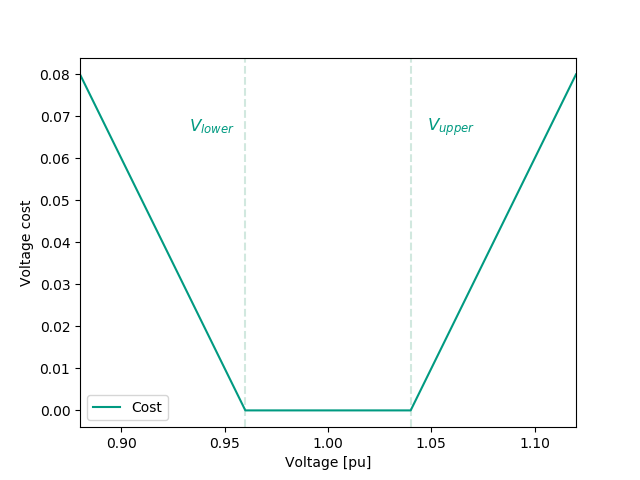
\includegraphics[height=8cm, width=12cm]{figures/voltage_cost.png}
    \caption[size = 9]{Voltage cost at a bus in the power system}
    \label{fig:problem:voltage_cost}
\end{figure}

Let $C_{current,i}$ be the cost of violating current margins in line $i$

\begin{equation}
   \begin{aligned}
   \label{eq:problem:current_margins_cost}
    C_{current,i} = \max(0,|I_{i}| - I_{upper})
    \end{aligned} 
\end{equation}
where $I_{upper}$ is the per unit upper current limit in lines. The current cost is plotted in figure  \ref{fig:problem:current_cost}.

\begin{figure}[ht]
    \center
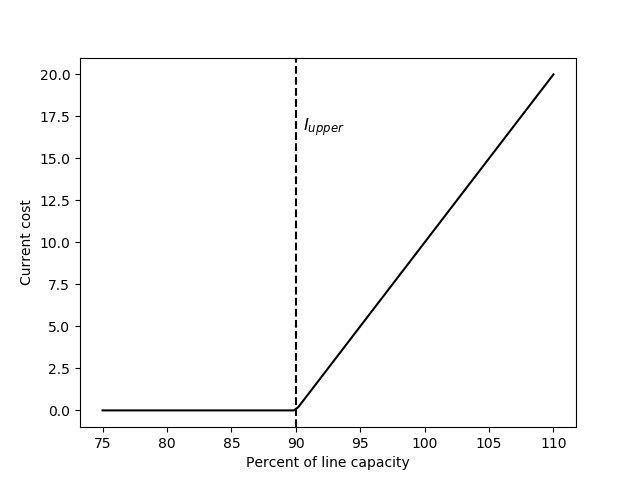
\includegraphics[height=8cm, width=12cm]{figures/current_cost.png}
    \caption[size = 9]{Current cost for a line in the power system}
    \label{fig:problem:current_cost}
\end{figure}

It is necessary to incentives costumers to offer flexibility in a realistic modelling of demand response. In other words, costumers should be economically compensated when their flexibility is activated. In classical incentive based programs (IBP) for demand control, costumers are given some sort of participation payment, such as a discount rate \cite{demand_response_definition}. On the other hand, marked based IBP compensates the costumers based on how much they participate. The most natural cost to consider in this thesis is the marked based IBP because the agent can continuously change the consumption of power at flexible loads. The activation cost $C_{activation,i}$ is defined as

\begin{equation}
   \begin{aligned}
   \label{eq:problem:activation_cost}
    C_{activation,i} = \lambda |\Delta P_{i}|
    \end{aligned} 
\end{equation}
where $|\Delta P_{i}|$  is the absolute change in power consumption at flexible load \textit{i} and $\lambda$ is the flexibility price at the time of activation.

It is desired that the flexible loads consume more power during periods with heavy solar production. In addition, flexible loads should use less energy during periods with low solar energy, so the total energy consumption in a day is not altered. However, the agent is not penalised during periods of low solar power production since there are no violations of current and voltage margins in the grid. As a result, there must be a signal that incentives the agent to reduce the power consumption in periods with low solar production. This could be done by be introducing the power imbalance $B_{i,t}$ of flexible load $i$ at time $t$.

\begin{equation}
   \begin{aligned}
   \label{eq:problem:balance}
    B_{i,t} = \sum_{k=1}^{24}\Delta P_{i,t-k}
    \end{aligned} 
\end{equation}
$\Delta P_{i,t-k}$ is the change in power consumption $k$ time steps before $t$ at flexible load \textit{i}. Simply put, the imbalance $B_{i,t}$ expresses if a flexible load is in balance in terms of energy consumption over the last 24 hours. A positive imbalance means the flexible loads have consumed more power than they originally planed. The goal is to have the imbalance close to zero, which means that power consumption has been shifted and not altered in absolute magnitude. The agent should be punished for having a large imbalance. Consequently, it should be penalised for taking an action that increases the absolute balance quantity. Let $C_{imbalance,i}$ be the energy imbalance cost at time $t$ for flexible load \textit{i}.

\begin{equation}
   \begin{aligned}
   \label{eq:problem:balance_cost}
    C_{imbalance,i} = |B_{i,t}| - |B_{i,t-1}|
    \end{aligned} 
\end{equation}
where the balance $B_{i,t}$ is given by equation \eqref{eq:problem:balance}. The agent is penalised if the result of an action increases the energy imbalance in absolute magnitude.  

The total cost of an agent at each step is defined as a linear combination over the voltage, current, activation and imbalance cost 

\begin{equation}
   \begin{aligned}
   \label{eq:problem:total_cost}
    C = 
    \kappa_{1} \sum_{i=1}^{F}C_{activation,i} + 
    \kappa_{2} \sum_{i=1}^{L}C_{current,i} +
    \kappa_{3} \sum_{i=1}^{N}C_{voltage,i} +
    \kappa_{4} \sum_{i=1}^{L}C_{imbalance,i} 
    \end{aligned} 
\end{equation}
Where \textit{L}, \textit{F} and \textit{N} are the number of lines, flexible loads and buses respectively. The weights $\kappa_{i}$ can be tuned, based on what the desired behaviour of the agent is. If safety margins are most important, the weights for cost of activation and imbalance should be small. Note that it is possible to discard a cost completely by setting its weight equal to zero. Lastly, the cost must be turned into a reward that a reinforcement algorithm can use. The reward $R$ is simply defined to be the negative of the cost

\begin{equation}
   \begin{aligned}
   \label{eq:problem:total_reward}
    R = - C
    \end{aligned} 
\end{equation}
where the total cost $C$ is defined by \eqref{eq:problem:total_cost}. Table \ref{table:reward_terms} summarises the different costs and their definition. 

\begin{table}[ht]
\centering
\caption{Cost terms that can be used in the reinforcement algorithm. The subscripts 'upper' and 'lower' means the upper and lower safety margins. $\lambda$ is the unit cost for activation of a flexible load ($\pounds/MWh$). $\Delta P_{i}$ is the change in consumption of flexible load \textit{i}. $B_{i,t}$ is the daily energy imbalance as defined in \eqref{eq:problem:balance}}
\label{table:reward_terms}
\begin{tabular}{l|ll}

Cost  & Definition & Comment
\\ 
\hline
Voltage &
$\max(0,|V_{i}| - V_{upper}) + \max(0,V_{lower}- |V_{i}|)$ &
Violation of voltage margin
\\
Current &
$\max(0,|I_{i}| - I_{upper})$&
Violation of current margin
\\
Activation &
$\lambda |\Delta P_{i}|$&
Activating flexibility
\\
Imbalance &
$|B_{i,t}|- |B_{i,t-1}|$&
Changing daily energy consumption
\\
\hline
\end{tabular}
\end{table}

\section{Playing an episode}
This section will describe how the the state of the electric grid is updated in an episode. The reinforcement agent is each hour given a state that represents the system, which includes a forecast for power demand and solar irradiance. Naturally, no forecasts are perfect, so the actual power demand and solar irradiance should deviate from the estimated values. This is done by adding a noise term to the forecasted values. The noise terms for the demand and solar irradiance are assumed to follow a Gaussian distribution with mean 0 and a standard deviation that is proportional to the forecast in that hour. The hyper parameters $\sigma_{solar}$ and $\sigma_{demand}$ determine the uncertainty in the forecasts, and the default values are set to 3 \% in both cases.



The reinforcement agent evaluates a state $s$ and picks an action $a$ to perform in each hour. The action determines the change in power consumption at the flexible loads in the power grid. The power flow equation are ready to be solved when the power demand resulting from the action is computed. There are no voltage regulating generators in the power grid that is used. Consequently, all the buses in the network are modelled as PQ-buses, except for the external grid (slack bus) where active power $P$ and voltage angle $\delta$ are known. After the power flow calculations have been performed, the reward is calculated and used to evaluate the action of the agent. Finally, the forecasts for demand and solar irradiance are updated and the state $s_{t+1}$ for the next hour is found. This concludes the processes involved in one time step of the reinforcement model. The learning process is summarised in pseudo code in algorithm \ref{problem:algorithm_playing_episode} 


\begin{algorithm}[H]
\SetAlgoLined
Select state space $\mathcal{S}$, flexibility $f \in [0,1]$, reward function $r$ 
 \\


 \For{episode 1:M}{
  Randomly select start day and start hour\\
  Receive initial state $s_{1}$
  
  \For{t 1:T}{
Let the reinforcement agent select an action $a_{t}$ based on $s_{t}$
\\
Set global solar irradiance $r$ based on forecasted solar irradiance $r_{forecast}$
\begin{equation}
   \begin{aligned}\label{eq:problem:set_solar_irradiance}
  r = r_{forecast} + \epsilon \cdot r_{forecast}, \;\; \epsilon \sim \mathcal{N}(0,\sigma_{solar})
    \end{aligned} 
\end{equation}

\For{Static generator 1:S}{
 Update solar production $P_{sun}$ based on nominal value $S_{N}$
\begin{equation}
   \begin{aligned}\label{eq:problem:set_solar}
  P_{sun} = r S_{N}
    \end{aligned} 
\end{equation}
} 

\For{Load 1:F}{
 Set power demand $P$ based on forecasted power demand $P_{forecast}$
\begin{equation}
   \begin{aligned}\label{eq:problem:set_demand_for}
  P = P_{forecast} + \epsilon \cdot P_{forecast}, \;\; \epsilon \sim \mathcal{N}(0,\sigma_{demand})
    \end{aligned} 
\end{equation}
}


\For{Flexible load 1:F}{
Update power demand $P$ based on the agent's action $a$ and flexibility $f$
\begin{equation}
   \begin{aligned}
   \label{eq:problem:update_demand_algorithm}
    P \leftarrow P + a f P_{forecast}
    \end{aligned} 
\end{equation}
}

Solve power flow equations
\\
Calculate reward with reward function $r$
\\
Find next state $s_{t+1}$


   }{
   
  }
 }
 \caption{Process for updating power demand and solar production in the electrical power grid}
 \label{problem:algorithm_playing_episode}
\end{algorithm}


\end{document}